\documentclass[11pt,titlepage,a4paper]{report}

%INCLUSIONE PACCHETTI
%---------------------------------------------
\usepackage[italian]{babel}
\usepackage{fancyhdr}
\usepackage{graphicx}
\graphicspath{{./pics/}}	% cartella di salvataggio immagini

% STILE DI PAGINA
%---------------------------------------------
\pagestyle{fancy}
\renewcommand{\sectionmark}[1]{\markright{\thesection.\ #1}}
\lhead{\nouppercase{\rightmark}}
\rhead{\nouppercase{\leftmark}}
\renewcommand{\chaptermark}[1]{%
\markboth{\thechapter.\ #1}{}}

%Ridefinisco lo stile plain della pagina
\fancypagestyle{plain}{%
	\lhead{
\includegraphics[height=50pt]{logo.eps}}
	\chead{}
	\rhead{HappyCode inc \\ happycodeinc@gmail.com}
	\lfoot{BR-jsys}
	\cfoot{\thepage}
	\renewcommand{\headrulewidth}{1pt}
	\renewcommand{\footrulewidth}{1pt}
}

%---------------------------------------------


%INIZIO DOCUMENTO


%---------------------------------------------
% PRIMA PAGINA
%---------------------------------------------
\begin{document}
\hyphenation{glos-sa-rio es-pli-ci-to ve-ri-fi-ca-re re-po-si-to-ry se-gna-la-ta coe-ren-za}
\begin{titlepage}
\begin{center}
\vspace*{0.5in}

\includegraphics{logo.eps}
\vspace*{0.2in}

{\Large \textbf{BR-jsys}}
{\Large \emph{business rules} per sistemi gestionali in architettura J2EE } 
\vspace{1.3in}
\par\rule{10cm}{.4pt} \par
\par\rule{12cm}{1pt} \par
\vspace*{0.5in}
\LARGE \textbf {ANALISI DEI REQUISITI}
\vspace*{0.5in}
\par\rule{12cm}{1pt} \par
{\large Versione 1.3 - \today}
\par\rule{10cm}{.4pt} \par

\end{center}
\end{titlepage}
\vspace*{0.5in}

%---------------------------------------------
% SECONDA PAGINA
%---------------------------------------------
\begin{center}
\thispagestyle{plain}
\begin{table}[htbp]
\large{
\begin{tabular}{l}
\Large{\textbf{\textsf{Capitolato: ''BR-jsys``}}} \\
\begin{tabular}{||p{6cm}||p{6cm}||}
\hline
\textbf{Data creazione:} & 18/11/2007 \\
\hline
\textbf{Versione:} & 1.3 \\
\hline
\textbf{Stato del documento:} & Formale, esterno \\
\hline
\textbf{Redazione:} & Michele Bortolato, 

Alessia Trivellato \\
\hline
\textbf{Revisione:} &   Marco Tessarotto \\
\hline
\textbf{Approvazione:}  & Elena Trivellato\\
\hline
\end{tabular} \\
\end{tabular}
}
\end{table}

\begin{table}[hbtp]
\large{
\begin{tabular}{l}
\Large{\textbf{\textsf{Lista di distribuzione}}} \\
\begin{tabular}{||p{6cm}||p{6cm}||}
\hline
{Elena Trivellato}& Responsabile di progetto \\ 
\hline 
{Filippo Carraro}& Progettista \\ 
\hline
{Alessia Trivellato, 

Michele Bortolato}& Analisti \\
\hline
{Marco Tessarotto}& Verificatore \\
\hline
{Tullio Vardanega,

Renato Conte}& Committente \\
\hline 
{Zucchetti S.r.l}& Azienda proponente\\
\hline
\hline
\end{tabular} \\
\end{tabular}
}
\end{table}

\begin{table}[hbtp]
\large{
\begin{tabular}{l}
\Large{\textbf{\textsf{Diario delle modifiche}}} \\
\begin{tabular}{||p{2cm}||p{3.5cm}||p{6cm}||}
\hline
\textbf{Versione} & \textbf{Data rilascio} & \textbf{Descrizione} \\
\hline
1.3 & 03/12/2007 & Correzioni grammaticali, correzioni strutturali.\\
\hline
1.2 & 28/11/2007 & Inserimento casi d'uso.\\
\hline
0.2 & 22/11/2007 & Aggiornamento requisiti. \\
\hline
0.1 & 18/11/2007 & Stesura preliminare del documento. \\
\hline

\end{tabular} \\
\end{tabular}

}
\end{table}
\end{center}
\newpage

\chapter*{Sommario} 
Il presente documento contiene una descrizione del prodotto oggetto del capitolato d'appalto designato dalla sigla BR-jsys. Tale descrizione comprende le sue funzionalit\`a, la tipologia di utenti ed il contesto d'uso. Prosegue con la descrizione e l'analisi dei requisiti del prodotto in questione con l'ausilio di un formalismo grafico: i diagrammi use-case UML. Vengono infine elencati tutti i requisiti individuati dalla HappyCode inc.

\tableofcontents
\chapter{Introduzione}
\section{Scopo del documento}
Il presente documento viene redatto al fine di identificare i requisiti impliciti ed espiciti presenti nel capitolato d'appalto denominato BR-jsys e pubblicato dal committente per conseguire il raggiungimento dell'obiettivo richiesto e soddisfare le esigenze di tutti gli stakeholders coinvolti nella realizzazione del progetto di cui sopra.
\section{Scopo del prodotto}
Il prodotto che verr\`a realizzato va inserito in un progetto globale. Il suo obiettivo principale \`e quello di integrare il sistema di validazione dei dati destinati al database dell'applicazione principale attraverso la creazione di business rules utili a confutarne la validit\`a ed evitare quindi l'introduzione di errori nel processo di acquisizione. Si tratta in sostanza di introdurre un nuovo strato applicativo che aiuti a realizzare la consistenza dei valori introdotti.
\section{Glossario}
Viene fornito come file esterno (Glossario\_0\_4.pdf).
\subsection{Definizioni, acronimi, abbreviazioni}
Per la visione dei suddetti contenuti si rimanda alla consultazione del glossario allegato. 
\section{Riferimenti}
Per un miglior tracciamento dei requisiti abbiamo ritenuto opportuno consultarci con l'azienda proponente. Il contenuto di tale contatto \`e reperibile nel verbale allegato (Incontro2007\_11\_22.pdf).
\section{Descrizione degli allegati}
Oltre al presente documento l'offerta \`e accompagnata dai seguenti allegati:
\begin{itemize}
\item Piano di Progetto: riporta l'impegno orario totale aziendale, l'impegno orario dei singoli componenti ed il costo preventivato.
\item{}Piano di Qualifica: definisce la strategia di verifica e validazione.
\item{}Glossario: definisce i termini non chiari e che assumono un significato particolare per il fornitore.
\end{itemize}
\chapter{Descrizione generale}
\section{Contesto di utilizzo}
Il prodotto richiesto dal cliente rientra nell'ambito di un progetto globale di automazione nella generazione del codice per la produzione di software gestionale. Il risultato di questo prodotto si traduce in piattaforme applicative complesse in ambiente J2EE che interagiscono con database relazionali. 
\section{Funzioni del prodotto}
Con la realizzazione del prodotto richiesto si vuole fornire uno strumento software idoneo a validare il processo di inserimento e di elaborazione dei dati che intercorre nel progetto globale. Verranno portate a termine alcune fasi intermedie:
\begin{itemize}
\item{}Definizione di un linguaggio semplice ed espressivo per definire le regole di validazione (business rules) e calcolo per classi business object;
\item{}realizzazione di un repository di regole in formato XML;
\item{}realizzazione di un validatore che verifichi staticamente la coerenza di suddette regole;
\item{}realizzazione di un interfaccia (API) per eseguire le regole di validazione e ottenere il risultato della valutazione, sia come accettazione dei valori inseriti, che come messaggi di errore da presentare all'utente;
\item{}realizzazione di un interprete dinamico che valuti le regole lette dal repository nel contesto della classe che realizza il business object e che indichi se \`e possibile proseguire con la transazione verso il database.
\end{itemize}
\section{Caratteristiche degli utenti}
Il prodotto \`e rivolto ad una fascia di utenza che non necessit\`a di particolari conoscenze informatiche ma esperta in ambito commerciale e gestionale. 
\section{Vincoli generali di utilizzo}
La piattaforma che andremo a realizzare si appoggia su di un server di tipo J2EE 2.5.
Il repository delle regole deve essere scritto secondo il linguaggio XML.
\section{Assunzioni e dipendenze}
\begin{itemize}
\item{}Le business rules sono divise in 3 tipi di classe fondamentali (rejector, projector, calculator);
\item{}la virtual machine utilizzata  per sviluppare gli oggetti richiesti \`e Java 1.5.
\end{itemize}
\chapter{Tabella dei requisiti}
\section{Requisiti funzionali}
\subsection{Obbligatori}
\begin{itemize}
\item[3.1.1.1]Il validatore statico deve poter verificare la coerenza delle regole: verificare cio\`e se esse costituiscono un insieme soddisfacilbile o se rigettano qualunque insieme di valori possibili per i business object. (R. ESPLICITO) 
\item[3.1.1.2]L'interprete dinamico associa classi java a regole. (R. ESPLICITO)
\item[3.1.1.3]L'interprete valuta le regole lette dal repository nel contesto della classe che realizza il business object e indica se \`e possibile proseguire con la transazione verso il database. (R. ESPLICITO)
\item[3.1.1.4]Deve essere possibile creare regole atte alla realizzazione di operazioni di calcolo a completamento di input parziali dell'utente. (R. ESPLICITO)
\item[3.1.1.5]I business object devono poter gestire oggetti di tipo Master, Detail o Master/Detail. (R. ESPLICITO)
\item[3.1.1.6]Deve essere possibile inserire e cancellare regole nel repository. (R. ESPLICITO)
\item[3.1.1.7]Violazioni di regole da parte dei business objects verranno gestiti mediante appropriata gestione degli errori. (R. ESPLICITO)
\item[3.1.1.8]Il contenuto del repository deve poter essere cambiato a run time senza dover procedere con nuova programmazione. (R. ESPLICITO)
\end{itemize}
\subsection{Opzionali}
\begin{itemize}
\item[3.1.2.1]Il prodotto dovrebbe essere dotato di un compilatore per tradurre le business rules in classi java, per non avere penalizzazioni in tempo di esecuzione. (R. ESPLICITO)
\end{itemize}
\section{Requisiti di qualit\`a}
\subsection{Obbligatori}
\begin{itemize}
\item[3.2.1.1]Definizione di un repository di regole in XML. (R. ESPLICITO)
\item[3.2.1.2]Realizzazione di un linguaggio di alto livello per definire le regole di validazione e calcolo per le classi java. (R. ESPLICITO)
\item[3.2.1.3]Il sistema di regole utilizzer\`a java reflection per le classi di business objects di cui \`e costituito. (R. ESPLICITO)
\item[3.2.1.4]Le business rules che implemeteremo saranno di tipo rejector. (R. ESPLICITO)
\item[3.2.1.5]Il progetto verr\`a accompagnato da una completa documentazione che descriver\`a:
\begin{itemize}
\item{}il linguaggio di definizione delle regole;
\item{}l'interazione con la classe java;
\item{}il repository delle regole;
\item{}l'API di attivazione delle regole;
\item{}l'interprete e validatore delle regole;
\end{itemize}\
(R. ESPLICITO)
\item[3.2.1.6]Al prodotto finale verr\`a allegato un manuale tecnico e la documentazione di accompagnamento del codice sorgente.(R. ESPLICITO)
\end{itemize}
\subsection{Desiderabili}
Il sistema dovrebbe: 
\begin{itemize}
\item[3.2.2.1]fornire elevata configurabilit\`a ed estendibilit\`a delle classi java; (R. ESPLICITO)
\item[3.2.2.2]aiutare gli utenti meno esperti a non commettere errori grossolani attraverso la verifica formale delle regole. (R. ESPLICITO)
\end{itemize}
\section{Requisiti di interfacciamento}
\subsection{Obbligatori}
\begin{itemize}
\item[3.2.3.1]Il linguaggio scelto deve essere di alto livello; (R. ESPLICITO)
\item[3.2.3.2]Il prodotto si deve integrare con le componenti gi\`a esistenti del progetto globale nell'ambito del quale verr\`a usato. (R. ESPLICITO)
\end{itemize}
%---------------------------------------------
\chapter{Casi d'uso}
\section{Validazione nuova business rule.}
\begin{center}
 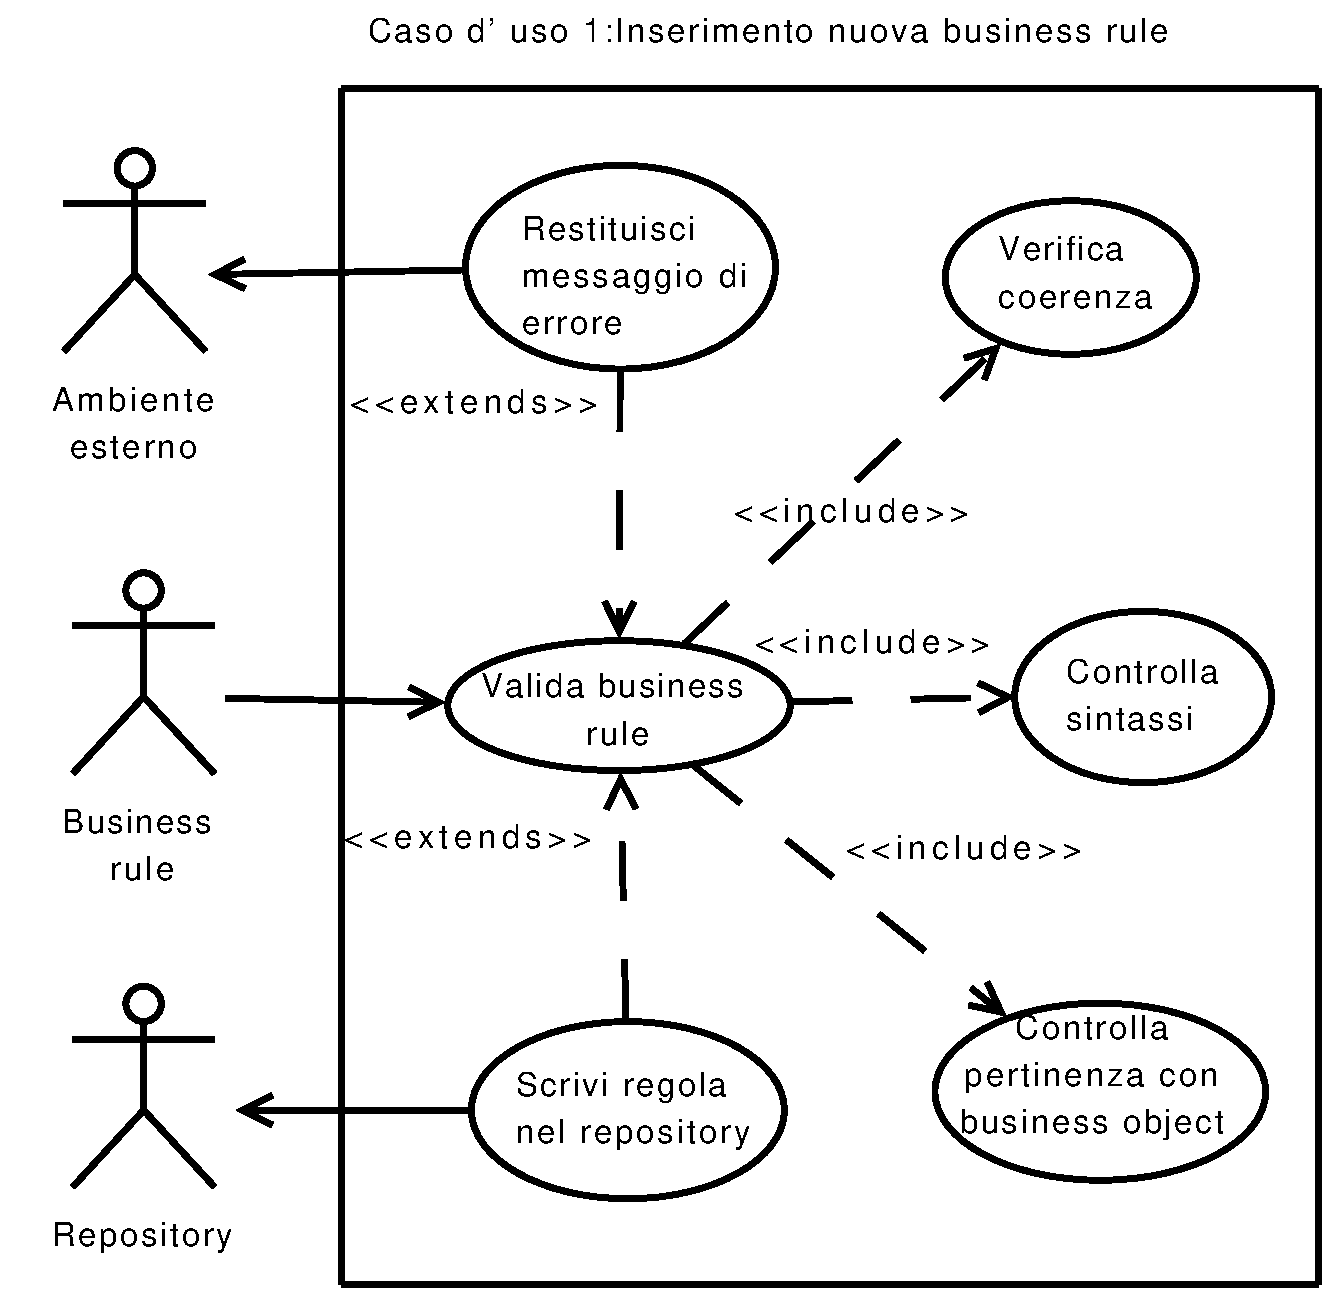
\includegraphics[width=0.8\textwidth]{Inserisci-regola.eps}
\end{center}

\begin{itemize}
\item{\textbf{Attori coinvolti:}}
\begin{itemize}
\item[-] business rule.
\item[-] repository.
\item[-] ambiente esterno.
\end{itemize}

\item{\textbf{Scopo e decrizione sintetica:}}\\
Il validatore riceve in ingresso una nuova business rule, che dovr\`a essere validata per essere scritta nel repository.

\item{\textbf{Flusso di eventi:}}
\begin{itemize}
 \item[-] Il validatore carica la business rule.
 \item[-] Viene fatto un controllo sintattico per verificare che la business rule sia espressa secondo il linguaggio  appropriato.
 \item[-] Si controlla che i campi ai quali vuole accedere la business rule combacino con quelli dei business objects.
 \item[-] Si effettua un controllo di coerenza con le altre regole presenti nel repository.
 \item[-] Si scrive la nuova business rule nel repository.
\end{itemize}

\item{\textbf{Precondizioni:}}\\
\`E stata immessa una nuova business rule.

\item{\textbf{Postcondizioni}}\\
La business rule viene scritta nel repository oppure viene segnalato l'errore all'ambiente esterno.

\end{itemize}

\subsection{Scrivere business rule nel repository.}

 \begin{itemize}
\item{\textbf{Attori coinvolti:}}
\begin{itemize}
\item[-] business rule.
\item[-] repository.
\item[-] ambiente esterno.
\end{itemize}
\item{\textbf{Scopo e decrizione sintetica:}}\\
La business rule viene scritta nel repository in maniera da facilitarne un suo uso successivo.
\item{\textbf{Flusso di eventi:}}
\begin{itemize}
 \item[-] Tramite metodi opportuni la business rule verr\`a scomposta e posta nel repository per una sua successiva applicazione.
 \item[-]L'ambiente esterno viene informato dell'avvenuto inserimento.
\end{itemize}
\item{\textbf{Precondizioni:}}\\
La business rule ha passato il test sintattico, di coerenza con gli oggetti business coinvolti e di coerenza con le altre regole business precendentemente presenti nel repository.
\item{\textbf{Postcondizioni:}}\\
Il repository contiene una nuova business rule.
\item\textbf{{Specifiche supplementari:}}\\
Si dovr\`a porre la nuova business rule nel repository in maniera che non sussistano ambiguit\`a con le altre gi\`a presenti.
Si dovranno comunque rispettare i criteri programmazione XML.

\end{itemize}
\subsection{Controllare sintassi.}
\begin{itemize}
\item{\textbf{Attori coinvolti:}}
\begin{itemize}
\item[-] business rule.
\item[-] ambiente esterno.
\end{itemize}
\item{\textbf{Scopo e decrizione sintetica:}}\\
Si controlla che la nuova business rule sia formulata secondo le specifiche del linguaggio scelto.
\item{\textbf{Flusso di eventi:}}
\begin{itemize}
 \item[-] Controllo sintassi per la nuova business rule.
\end{itemize}
\item{\textbf{Precondizioni:}}\\
\`E stata immessa una nuova business rule.
\item{\textbf{Postcondizioni:}}\\
La business rule pu\`o avanzare al controllo di coerenza con gli oggetti business oppure viene segnalata un'anomalia all'ambiente esterno.

\end{itemize}
\subsection{Controllare pertinenza con business object.}
\begin{itemize}
\item{\textbf{Attori coinvolti:}}
\begin{itemize}
\item[-] business rule.
\item[-] ambiente esterno.
\end{itemize}
\item{\textbf{Scopo e decrizione sintetica:}}\\
Si controlla che la nuova business rule si riferisca a campi dato pertinenti agli oggetti business coinvolti.
\item{\textbf{Flusso di eventi:}}
\begin{itemize}
 \item[-] Contollo pertinenza con oggetti business coinvolti.
\end{itemize}
\item{\textbf{Precondizioni:}}\\
La nuova business rule ha superato positivamente la validazione sintattica.
\item{\textbf{Postcondizioni:}}\\
La nuova business rule pu\`o avanzare al controllo di coerenza con gli altri oggetti business presenti nel repository oppure viene segnalato un errore all'ambiente esterno.
\item\textbf{{Specifiche supplementari:}}\\
Saranno necessarie tecniche specifiche di accesso agli oggetti business coinvolti.
\end{itemize}
\subsection{Controllare coerenza.}
\begin{itemize}
\item{\textbf{Attori coinvolti:}}
\begin{itemize}
 \item[-] business rule.
 \item[-] ambiente esterno.
\end{itemize}
\item{\textbf{Scopo e decrizione sintetica:}}\\
Si controlla la coerenza della nuova business rule con le altre regole business presenti nel repository.
\item{\textbf{Flusso di eventi:}}
\begin{itemize}
\item[-] Controllo coerenza con le altre regole business presenti nel repository.
\end{itemize}
\item{\textbf{Precondizioni:}}\\
La nuova business rule ha superato positivamente il controllo di pertinenza con gli oggeti business coinvolti.
\item{\textbf{Postcondizioni:}}\\
La nuova business rule viene scritta nel repository oppure viene segnalata un'anomalia all'ambiente esterno.
\item\textbf{{Specifiche supplementari:}}\\
Le regole business presenti nel repository possono essere molte, ma non tutte si riferiscono agli stessi oggetti business, il controllo di coerenza dovr\`a essere intelligente, dovr\`a fare il controllo solo sulle regole che possono effettivamente andare in conflitto con la nuova,infine la business rule dovr\`a essere posta nel repository in modo da permettere un analisi il pi\`u efficiente possibile.

\end{itemize}
\subsection{Restituire messaggi di errore.}
\begin{itemize}
\item{\textbf{Attori coinvolti:}}
\begin{itemize}
\item[-]  business rule.
\item[-] ambiente esterno.
\end{itemize}
\item{\textbf{Scopo e decrizione sintetica:}}\\
In caso di fallimento nella validazione verr\`a avvisato in maniera opportuna l'ambiente esterno.
\item{\textbf{Flusso di eventi:}}
\begin{itemize}
 \item[-] Invia all'ambiente esterno un messagio che mostri in che punto della business rule si \`e verificato l' errore.
\end{itemize}
\item{\textbf{Precondizioni:}}\\
La nuova business rule non ha passato uno dei tre controlli di validazione.
\item{\textbf{Postcondizioni:}}\\
L'errore \`e stato segnalato correttamente.
\end{itemize}
\section{Esecuzione business rule.}
\begin{center}
 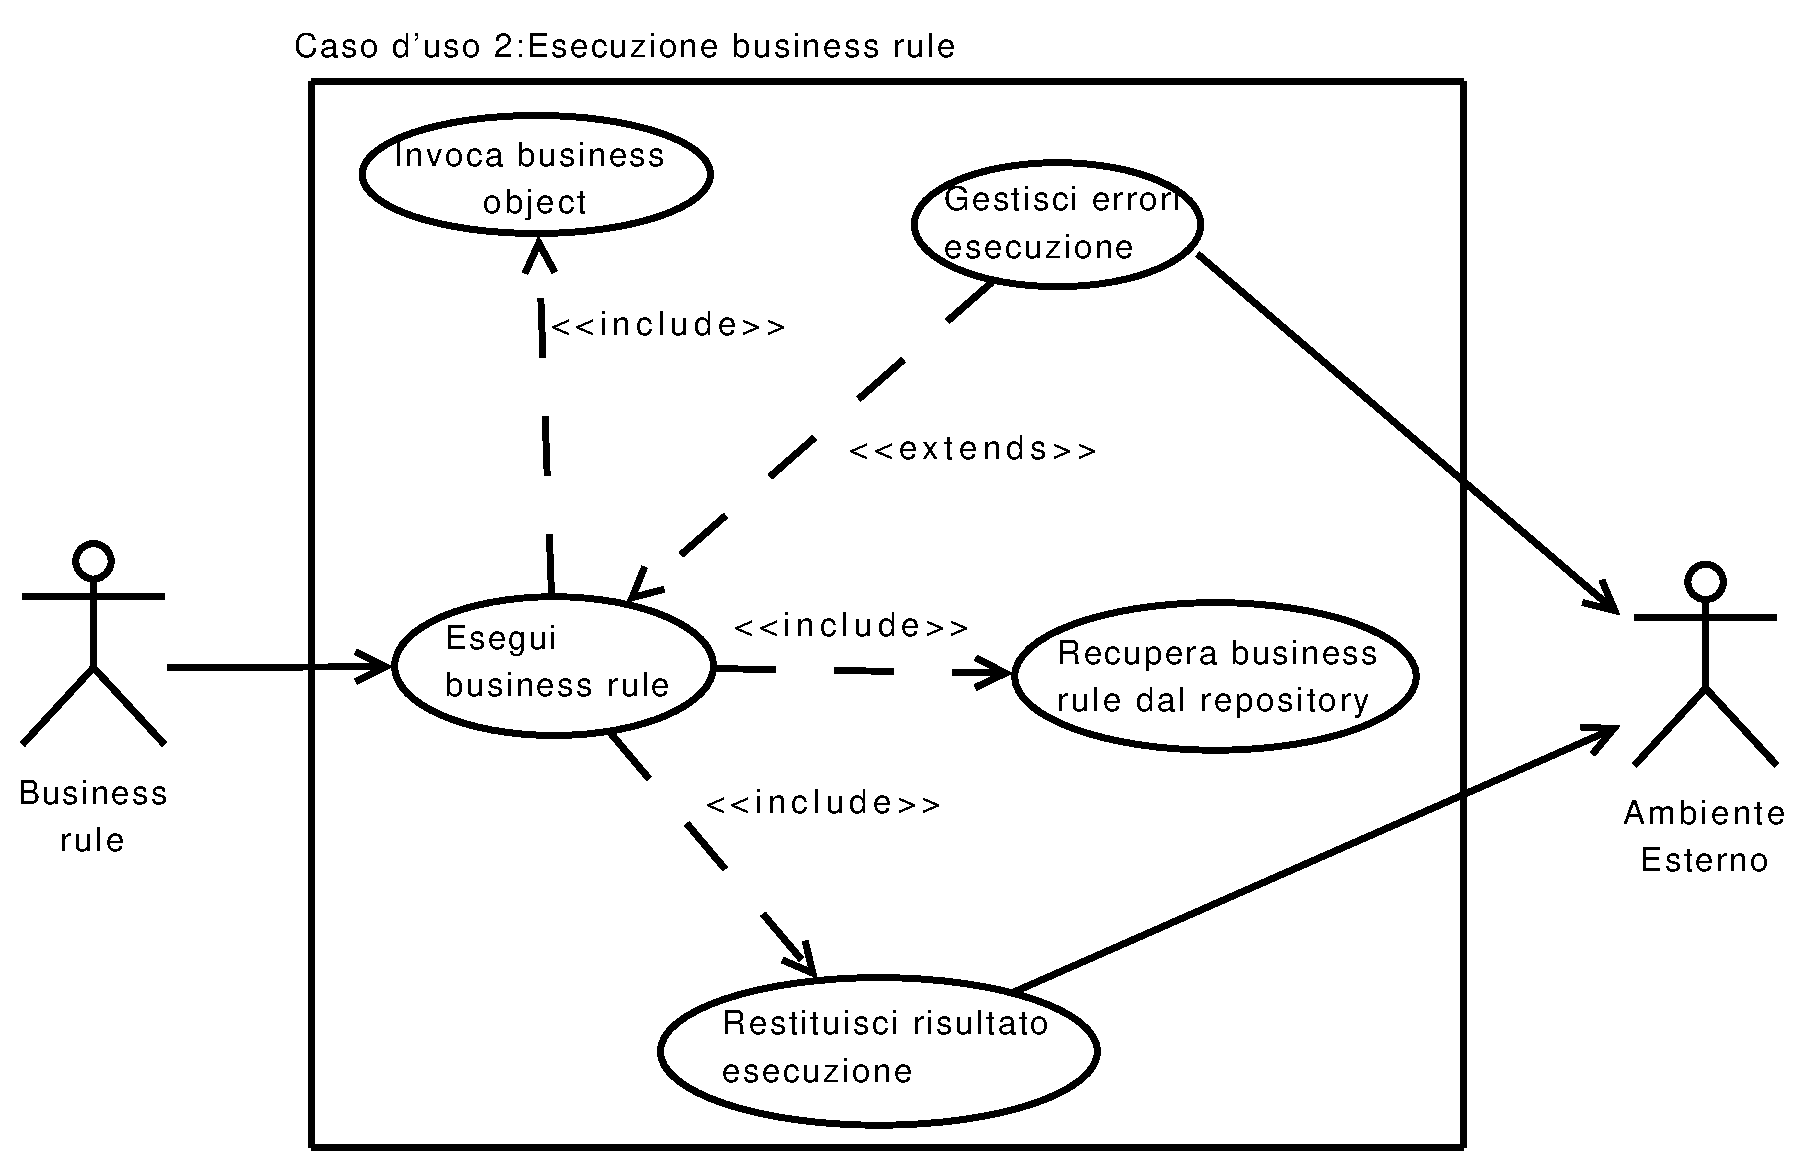
\includegraphics[width=1\textwidth]{Esegui-regola.eps}

\end{center}

\subsection{Eseguire business rule.}
\begin{itemize}
\item{\textbf{Attori coinvolti:}}
\begin{itemize}
\item[-] business rule.
\item[-] ambiente esterno.
\end{itemize}
\item{\textbf{Scopo e decrizione sintetica:}}\\
Le business rules presenti nel repository dovranno interagire con i business objects necessari. Successivamente si dovr\`a segnalare all'ambiente esterno l'esito della validazione.
\item{\textbf{Flusso di eventi:}}
\begin{itemize}
 \item[-] {La business rule viene recuperata dal repository.}
 \item[-] {Vengono invocati gli oggetti business necessari.}
 \item[-] {La business rule viene fatta eseguire.}
 \item[-] {Viene restituito il risultato del checking.}
\end{itemize}
\item{\textbf{Precondizioni:}}\\
\`E stata invocata una business rule.
\item{\textbf{Postcondizioni:}}\\
Il checking \`e stato effettuato.
\item\textbf{{Specifiche supplementari:}}\\
Il checking pu\`o dare esito positivo o negativo; possono tuttavia verificarsi degli errori eccezzionali che dovranno essere segnalati opportunamente.
\end{itemize}
\subsection{Recuperare business rule dal repository.}
\begin{itemize}
\item{\textbf{Attori coinvolti:}}
\begin{itemize}
\item[-] business rule.
\item[-] ambiente esterno.
\end{itemize}
\item{\textbf{Scopo e decrizione sintetica:}}\\
Data la richiesta d'uso di una business rule,la si dovr\`a cercare e recuperare dal repository XML.
\item{\textbf{Flusso di eventi:}}
\begin{itemize}
 \item[-] Rintraccia la business rule nel repository.
\end{itemize}
\item{\textbf{Precondizioni:}}\\
\`E avventuta la richiesta d'uso di una business rule.
\item{\textbf{Postcondizioni:}}\\
La business rule viene recuperata dal repository XML.
\item\textbf{{Specifiche supplementari:}}\\
Nel caso in cui la business rule non fosse presente, un opportuno avviso verrebbe segnalato all'ambiente esterno.
\end{itemize}
\subsection{Invocare business objects necessari.}
\begin{itemize}
\item{\textbf{Attori coinvolti:}}
\begin{itemize}
\item[-] business rule.
\item[-] ambiente esterno.
\end{itemize}
\item{\textbf{Scopo e decrizione sintetica:}}\\
Data la business rule dovr\`o invcare gli opportuni oggetti business.
\item{\textbf{Flusso di eventi:}}
\begin{itemize}
 \item[-] {Rintraccia gli oggetti business necessari.}
 \item[-] {Invoca gli oggetti business necessari.}
\end{itemize}
\item{\textbf{Precondizioni:}}\\
\`E stata recuperata una business rule dal repository.
\item{\textbf{Postcondizioni:}}\\
I business objects opportuni sono stati invocati.
\item\textbf{{Specifiche supplementari:}}\\
Nel caso in cui un business(oppure parte di esso) non fosse presente, verrebbe segnalata l'anomalia all'ambiente esterno.
\end{itemize}
\subsection{Restituire risultato del checking.}
\begin{itemize}
\item{\textbf{Attori coinvolti:}}
\begin{itemize}
\item[-] business rule.
\item[-] ambiente esterno.
\end{itemize}
\item{\textbf{Scopo e decrizione sintetica:}}\\
Verr\`a restituito all' ambiente esterno il risultato del check.
\item{\textbf{Flusso di eventi:}}
\begin{itemize}
 \item[-] {Restituire all'ambiente esterno il risultato del check.}
\end{itemize}
\item{\textbf{Precondizioni:}}\\
L'opportuna business rule \`e stata recuperata.
Gli opportuni oggetti business sonon stati invocati.
\item{\textbf{Postcondizioni:}}\\
L'ambiente esterno ha ricevuto l'esito del checking.

\end{itemize}
\subsection{Gestire errori esecuzione.}
\begin{itemize}
\item{\textbf{Attori coinvolti:}}
\begin{itemize}
 \item[-] business rule.
 \item[-] ambiente esterno.
\end{itemize}
\item{\textbf{Scopo e decrizione sintetica:}}\\
Segnala anomalie nelle funzionalit\'a precedentemente descritte.
\item{\textbf{Flusso di eventi:}}
\begin{itemize}
 \item[-] {Segnala anomalie avvenute in una delle funzionalit\`a sopra citate.}
\end{itemize}
\item{\textbf{Precondizioni:}}\\
Immessa la richiesta di esecuzione di una business rule.
\item{\textbf{Postcondizioni:}}\\
L'ambiente esterno \`e stato informato dell'anomalia.
\item\textbf{{Specifiche supplementari:}}\\
L'anomalia segnalata dovr\`a segnalare precisamente le caratteristiche di quest'ultima.
\end{itemize}
\end{document}
